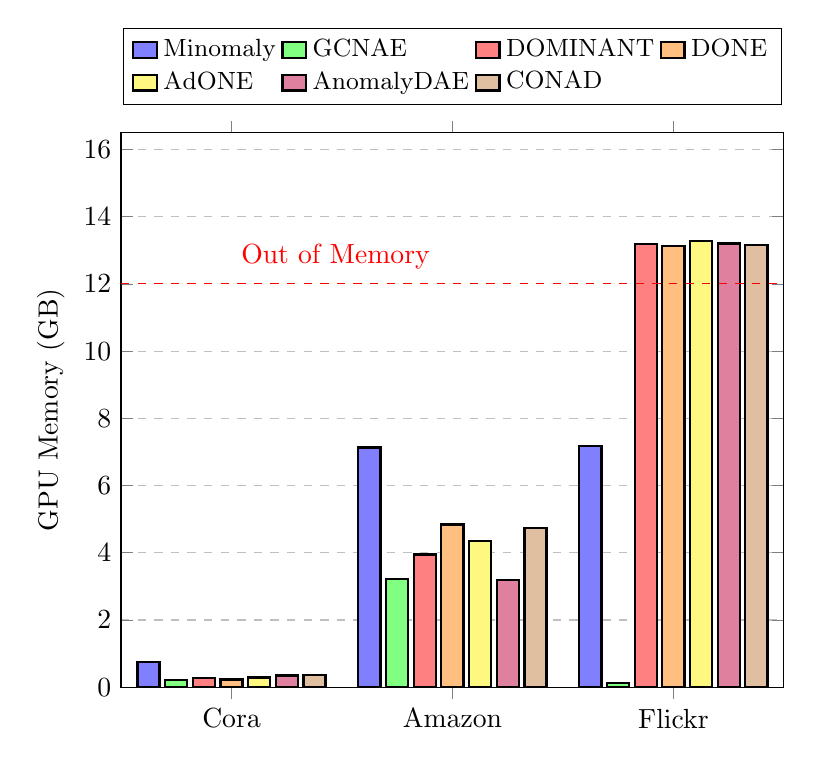
\begin{tikzpicture}
    \begin{axis}[
        ybar,
        bar width=8pt,
        width=10cm,
        enlargelimits=0.25,
        legend style={
            font=\small,
            at={(0.5,1.05)},
            anchor=south,
            legend columns=4
        },
        legend image code/.code={
            \draw [#1] (0cm,-0.1cm) rectangle (0.3cm,0.1cm);
        },
        ylabel={GPU Memory (GB)},
        symbolic x coords={Cora, Amazon, Flickr},
        xtick=data,
        ymin=0,
        ymax=15,
        enlarge y limits={upper=0},
        ymajorgrids=true,
        grid style=dashed,
        legend cell align=left,
        clip=false,
        % ---------------------------------------------------------------------
        % added stuff
        % ---------------------------------------------------------------------
        % allow different layers
        set layers,
        % (needed because of bug <https://sourceforge.net/p/pgfplots/bugs/153/>)
        cell picture=true,
        % now add the "horizontal line" ...
        extra y ticks=12,
        % ... don't show any label and ...
        extra y tick labels={},
        % ... adapt the style to your needs
        extra y tick style={
            % in case you should remove the grid from the "normal" ticks ...
            ymajorgrids=true,
            % ... but don't show an extra tick (line)
            ytick style={
                /pgfplots/major tick length=0pt,
            },
            grid style={
                red,
                dashed,
                % to draw this line before the bars, move it a higher layer
                /pgfplots/on layer=axis foreground,
            },
        },
        % ---------------------------------------------------------------------
        % moved common options from the `\addplot' commands here
        mark=none,
        error bars/y dir=both,
        error bars/y explicit,
        error bars/error bar style={
            thick,
        },
        after end axis/.code={
            \node[anchor=west, text=red] at (axis cs:Cora,12) [yshift=10pt] {Out of Memory};
        }
    ]

    \addplot[fill=blue!50, draw=black, thick] coordinates {
        (Cora,0.76) (Amazon,7.13) (Flickr,7.17)
    };
    \addlegendentry{Minomaly}

    \addplot[fill=green!50, draw=black, thick] coordinates {
        (Cora,0.22) (Amazon,3.22) (Flickr,0.12)
    };
    \addlegendentry{GCNAE}

    \addplot[fill=red!50, draw=black, thick] coordinates {
        (Cora,0.27) (Amazon,3.95) (Flickr,13.18)
    };
    \addlegendentry{DOMINANT}

    \addplot[fill=orange!50, draw=black, thick] coordinates {
        (Cora,0.23) (Amazon,4.84) (Flickr,13.12)
    };
    \addlegendentry{DONE}

    \addplot[fill=yellow!50, draw=black, thick] coordinates {
        (Cora,0.29) (Amazon,4.34) (Flickr,13.27)
    };
    \addlegendentry{AdONE}

    \addplot[fill=purple!50, draw=black, thick] coordinates {
        (Cora,0.35) (Amazon,3.19) (Flickr,13.20)
    };
    \addlegendentry{AnomalyDAE}

    \addplot[fill=brown!50, draw=black, thick] coordinates {
        (Cora,0.36) (Amazon,4.74) (Flickr,13.16)
    };
    \addlegendentry{CONAD}

    \end{axis}
\end{tikzpicture}